\documentclass[runningheads]{llncs}

\usepackage[T1]{fontenc}
\usepackage{lmodern}
\usepackage{graphicx}
\graphicspath{{images/}{./}}
\usepackage{tikz}
\usetikzlibrary{shapes,arrows.meta,positioning,calc}
\usepackage{booktabs}
\usepackage{amsmath}
\usepackage{amssymb}
\usepackage{hyperref}
\usepackage[none]{hyphenat}
\sloppy

\begin{document}

\title{Benchmarking Activity and Distortion Classification on Authentically
Distorted Surveillance Videos Using Handcrafted Trajectory Features}

\titlerunning{Classification Benchmarking on Authentically Distorted Surveillance Videos}

\author{Author Name Removed for Review}
\institute{Institution Removed for Review}

\maketitle

% ============================================================
\begin{abstract}
Real-world surveillance footage is frequently affected by authentic camera distortions, such as defocus blur and exposure variation, rarely represented in existing activity-recognition benchmarks. The Authentically Distorted Surveillance Videos (AD-SVD) dataset was introduced for object tracking under these conditions, but its suitability for supervised classification has not been explored. We reformulate AD-SVD as a benchmark for activity and distortion classification and test the hypothesis that, under authentic distortion, foreground detection quality, not classifier choice, limits downstream accuracy. A fixed-threshold detector recovers usable trajectories from only 46.5\% of the dataset; a confidence-driven adaptive detection method raises this to 99.7\%, increasing LightGBM accuracy from 69.4\% to 75.5\% for activity recognition and from 65.6\% to 97.7\% for distortion classification under stratified 5-fold cross-validation. Enriching preprocessing and features without fixing detection does not recover this loss. These results establish AD-SVD as a reproducible classification benchmark and show that trajectory recovery, not classifier sophistication, is what reliable recognition under authentic distortion depends on.

\keywords{Video Surveillance \and Activity Recognition \and Authentically Distorted Surveillance Videos \and Machine Learning}
\end{abstract}

% ============================================================
\section{Introduction}

Automated activity recognition increasingly compensates for the limits of manual surveillance monitoring~\cite{article}. Deep learning dominates large-scale benchmarks~\cite{ur2023use}, but its need for extensive labelled data and heavy computation makes handcrafted trajectory representations attractive for resource-constrained deployments~\cite{csurka2018handcrafted}. These representations, however, depend on reliable foreground extraction, which authentic distortions such as defocus blur and exposure variation are known to degrade~\cite{gillani2025distortion}. This dependence makes authentically distorted surveillance datasets particularly valuable for understanding where activity-recognition pipelines fail.

AD-SVD~\cite{9698081} was built to evaluate object tracking under exactly these distortions, using eight activities recorded across multiple cameras and locations under clean and distorted conditions. Its value for tracking is established, but whether it can support supervised classification, and what limits accuracy when used that way, has not been examined.

We hypothesize that under authentic distortion, foreground detection quality, not classifier or feature choice, sets the ceiling on classification accuracy, and test this directly. The contributions of this work are threefold: (i) reformulating AD-SVD as a benchmark for activity and distortion classification, (ii) isolating the influence of foreground detection from classifier and feature selection through controlled experiments, and (iii) introducing a confidence-driven Adaptive MOG2 detector that raises trajectory recovery from 46.5\% to 99.7\% and, consequently, downstream classification performance.

% ============================================================
\section{Related Work}

Handcrafted trajectory representations remain attractive for surveillance: interpretable, data-efficient, and competitive in resource-constrained settings~\cite{ahmed2018trajectory,csurka2018handcrafted}. Deep architectures achieve state-of-the-art results on large-scale benchmarks~\cite{ur2023use}, but their data and compute requirements limit applicability where labelled surveillance data are scarce.

Little work examines how authentic, in-capture distortions affect downstream classification: most benchmarks use synthetic degradations or favourable conditions, whereas real defocus blur and exposure variation degrade the foreground quality that motion-based features depend on~\cite{gillani2025distortion}. Gomez-Nieto et al.~\cite{9698081} introduced AD-SVD from a tracking perspective; whether the same detection difficulty limits supervised classification, and whether classifier or feature selection can compensate for it, remains unknown. This paper addresses that gap.

% ============================================================
\section{Methodology}

The pipeline transforms raw video into activity and distortion predictions through five stages (Fig.~\ref{fig:pipeline}): distortion-aware preprocessing, adaptive foreground detection, IoU--Hungarian tracking, multi-family feature blending, and classification, designed to isolate the influence of foreground detection quality on downstream performance.

\begin{figure}[htbp]
\centering
\resizebox{0.92\textwidth}{!}{%
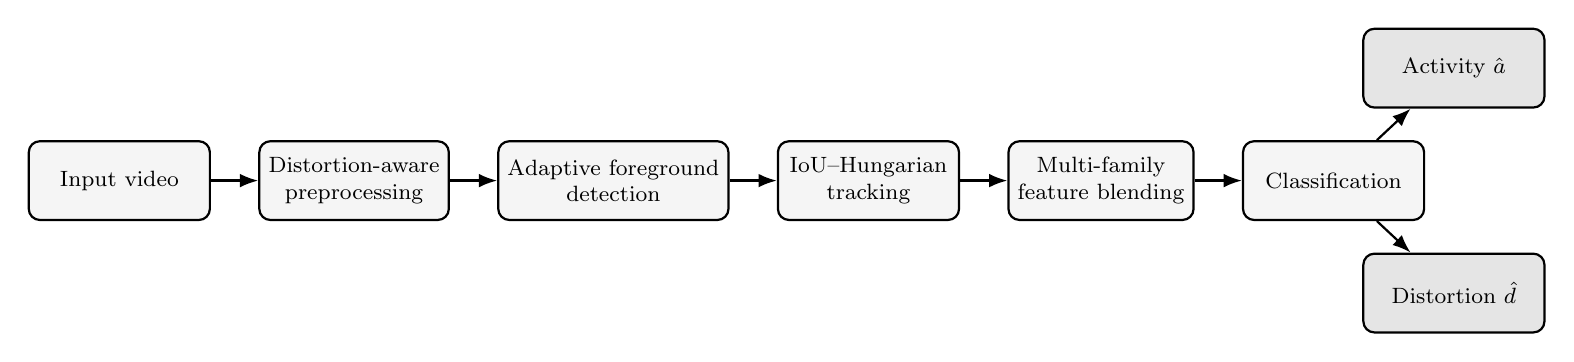
\begin{tikzpicture}[
  node distance=6mm,
  every node/.style={font=\footnotesize},
  box/.style={draw, rounded corners, fill=gray!8, minimum width=2.3cm,
              minimum height=1.0cm, align=center, thick},
  outbox/.style={box, fill=gray!20}
]
\node[box] (v) {Input video};
\node[box, right=of v] (pre) {Distortion-aware\\preprocessing};
\node[box, right=of pre] (det) {Adaptive foreground\\detection};
\node[box, right=of det] (trk) {IoU--Hungarian\\tracking};
\node[box, right=of trk] (feat) {Multi-family\\feature blending};
\node[box, right=of feat] (clf) {Classification};
\node[outbox, above right=4mm and -8mm of clf] (act) {Activity $\hat{a}$};
\node[outbox, below right=4mm and -8mm of clf] (dist) {Distortion $\hat{d}$};

\draw[-{Latex}, thick] (v) -- (pre);
\draw[-{Latex}, thick] (pre) -- (det);
\draw[-{Latex}, thick] (det) -- (trk);
\draw[-{Latex}, thick] (trk) -- (feat);
\draw[-{Latex}, thick] (feat) -- (clf);
\draw[-{Latex}, thick] (clf) -- (act);
\draw[-{Latex}, thick] (clf) -- (dist);
\end{tikzpicture}%
}
\caption{\textbf{Overview of the proposed classification pipeline.} Each stage transforms the previous stage's output into a more compact representation for classification.}
\label{fig:pipeline}
\end{figure}

Frames are resized and corrected for blur and exposure abnormalities before detection. Foreground segmentation uses MOG2 with a nominal variance threshold; each frame's mask is scored on coverage, fragmentation, and blob size, and combined with a track-quality prior into a confidence score $Q$. When $Q$ falls below a threshold, detection re-runs at a relaxed threshold, keeping the re-run mask only if it improves the score. This confidence-driven relaxation, Adaptive MOG2, is the paper's central methodological contribution. Detected regions are associated across frames via IoU-matching solved with the Hungarian algorithm, keeping trajectories longer than 30 frames.

Each trajectory is represented using handcrafted trajectory, kinematic, shape, and interaction descriptors, complemented by HOG and LBP appearance features computed independently of tracking success; per-video statistics are aggregated into a fixed-length feature vector. Five classifiers (Random Forest, SVM, KNN, LightGBM, XGBoost) are evaluated under identical stratified 5-fold cross-validation splits. To isolate the source of any gains, we compare a fixed-threshold \emph{baseline}, an \emph{ablation} adding richer preprocessing and features but keeping fixed-threshold detection, and the \emph{proposed} pipeline with Adaptive MOG2.

% ============================================================
\section{Experimental Evaluation}

AD-SVD contains 4,476 surveillance videos spanning eight activity classes recorded under four distortion conditions (Pristine, Exposure, Focus, Exposure+Focus) across four cameras and seven locations~\cite{9698081}. All experiments use stratified 5-fold cross-validation with identical fold partitions across configurations; accuracy (mean $\pm$ std.) is the primary metric, with weighted F1 as a complementary measure. Videos yielding no valid trajectory are excluded from the corresponding task, so trajectory yield is itself an evaluation outcome.
\begin{table}[htbp]
\centering
\caption{\textbf{Key results by configuration} (5-fold cross-validation, best classifier per configuration). Baseline: fixed-threshold MOG2. Ablation: fixed-threshold MOG2 with richer preprocessing/features. Proposed: Adaptive MOG2.}
\label{tab:key}
\resizebox{\textwidth}{!}{%
\begin{tabular}{lcccc}
\toprule
\textbf{Configuration} & \textbf{Trajectory yield} & \textbf{Best classifier} & \textbf{Activity Acc.} & \textbf{Distortion Acc.} \\
\midrule
Baseline & 46.5\% & LightGBM & 69.4\%$\pm$2.1 & 65.6\%$\pm$2.2 \\
Ablation & 51.4\% & LightGBM & 62.9\%$\pm$2.5 & 60.6\%$\pm$2.4 \\
\textbf{Proposed} & \textbf{99.7\%} & \textbf{LightGBM} & \textbf{75.5\%$\pm$0.7} & \textbf{97.7\%$\pm$0.5} \\
\bottomrule
\end{tabular}%
}
\end{table}

Table~\ref{tab:key} summarises the outcome. Adaptive detection raises trajectory yield from 46.5\% to 99.7\%, closing almost the entire gap left by the fixed-threshold detector. Enriching preprocessing and features alone, without fixing detection, raises yield only marginally (to 51.4\%) and reduces accuracy relative to the plain baseline, since the added feature dimensions are computed from the same short, fragmented trajectories. Adaptive detection instead drives a 6.1-point gain in activity accuracy and a 32.1-point gain in distortion accuracy over the strongest baseline classifier ($p=0.005$, paired $t$-test). Classifier choice matters far less: under the proposed configuration, LightGBM, XGBoost, and Random Forest differ by only a few percentage points, a spread small compared to the gap between configurations. Trajectory-derived motion statistics alone, with no explicit image-quality analysis, also separate the four distortion classes with high accuracy once yield is near-complete. This confirms the paper's hypothesis: detection quality, not classifier or feature sophistication, is the dominant factor limiting classification accuracy under authentic distortion.

% ============================================================
\section{Conclusion}

This work reformulates AD-SVD, originally developed for tracking evaluation, as a benchmark for supervised activity and distortion classification and shows that foreground detection quality, not classifier or feature sophistication, is what limits accuracy under authentic distortion. A confidence-driven adaptive detector raises trajectory yield from 46.5\% to 99.7\%, enabling LightGBM to reach 75.5\%$\pm$0.7 activity and 97.7\%$\pm$0.5 distortion accuracy. At the current dataset scale, handcrafted trajectory and appearance representations provide a strong, data-efficient baseline. Future work will investigate more advanced trajectory generation methods and larger-scale datasets to determine whether this dependence on foreground detection persists under increasingly challenging conditions.

% ============================================================
\begingroup
\small
\bibliographystyle{splncs04}
\bibliography{paper_references}
\endgroup

\end{document}